\chapter{Validación de la solución}\label{chap:3}

En el presente capítulo se detallará el procedimiento llevado a cabo para la aplicación de los algoritmos de minería de datos que se utilizarán para la obtención de reglas y clasificaciones, al igual que el proceso para construir los modelos descriptivos y predictivos para conocer el comportamiento de las transacciones bancarias.

\section{Algoritmos de aprendizaje supervisado}

El aprendizaje supervisado es una tarea en la que una computadora aprende una función que asigna entradas a salidas, en función de un conjunto de datos de pares de entrada y salida. Hay múltiples tareas bajo aprendizaje supervisado, y una de ellas es la clasificación. A continuación se presentan los algoritmos empleados en esta tarea.

\subsection{Clasificación}

La técnica de clasificación se utilizará con el propósito de, a partir de una base de datos de entrenamiento, evaluar el comportamiento de las transacciones de la base de datos de prueba. Para esta evaluación, se utilizan dos algoritmos de minería de datos: árboles de decisión y bosques aleatorios.

\subsubsection{Modelo de árbol de decisión}
Para la creación del modelo de árbol de decisión es utilizado el nodo \textit{Decision Tree}. Este construye el árbol utilizando variables numéricas y nominales. En este estudio se emplearon dos combinaciones de datos. Primero, se utilizan todas las variables obtenidas en la vista minable, y posteriormente se realiza una selección de atributos para realizar una comparación con respecto a la calidad de los resultados. \\
Se configura el nodo para obtener un árbol no binario, no podado y no colapsado, donde la variable objetivo es \textsf{is\_fraud}, que es un atributo nominal, y el número mínimo por registros por nodo es 100. Esta configuración aparece representada en la figura \ref{fig:config-decision-tree}. 

\begin{figure}[H]
	\centering
	\includegraphics[width=0.37\linewidth]{figuras/Ray/Arbol de decision/Configuracion del nodo Decision Tree}
	\caption{Configuración del nodo \textit{Decision Tree}}
	\label{fig:config-decision-tree}
\end{figure}

Se realiza una prueba con todas las variables resultantes de la vista minable obtenida en el capítulo \ref{chap:2}, y con el grupo con mejores resultados arrojados compuesto por las variables \textsf{category, amt, gender, state, is\_ fraud, Time y Age}. \\

\textbf{Resultados del algoritmo Decision Tree} \\
En la sección de anexos \ref{anex}, se presentan dos histogramas con las clasificaciones de las transacciones tras la ejecución del nodo \textit{Decisión Tree}. En el anexo \ref{aped.hist-all-des-tree}, se muestran los resultados con todas las variables obtenidas de la vista minable, donde se obtiene una clasificación de 1 575 transacciones fraudulentas y 554 144 transacciones lícitas. Mientras, en el anexo \ref{aped.hist-mejores-dt}, se presenta el resultado de la prueba con el grupo de variables con mejores resultados, donde se obtienen 1 720 transacciones fraudulentas y 553 999 transacciones lícitas. \\
En la figura \ref{fig:matriz-dec-tree} se muestran las matrices de confusión de la prueba con todos los datos, así como de la prueba con el grupo de variables con mejores resultados.

\begin{figure} [!h]
	\centering
	\begin{subfigure}[b]{0.49\linewidth}
		\includegraphics[width=\linewidth]{"figuras/Ray/Arbol de decision/Todas las variables/Matriz de confusion del nodo Score de arbol"}
		\caption{Con todas las variables de la vista minable}
		\label{fig:matriz-score-de-arbol}
	\end{subfigure}
\hfill
\begin{subfigure}[b]{0.49\linewidth}
	\includegraphics[width=\linewidth]{"figuras/Ray/Arbol de decision/Grupo de datos Mejores Resultados/Matriz de confusion del nodo Score de arbol"}
	\caption{Tras la elección de variables}
	\label{fig:matriz-dectree-best-}
\end{subfigure}
\caption{Resultados de la matriz de confusión tras ejecutar el nodo \textit{Decision Tree}}
\label{fig:matriz-dec-tree}
\end{figure}

Los resultados de la clasificación de las transacciones se muestran en la tabla \ref{tabla:res-desicion-tree}.

\begin{table} [H]
	\centering
	\begin{tabular}{p{6cm} | l | l}
		\toprule
		 & Todas las variables & Variables seleccionadas \\
		 \midrule
		Transacciones fraudulentas en la base de datos de prueba &	2145 & 2145 \\
		\hline
		Predicción de las transacciones fraudulentas (\% del total) &	1575 (73.43\%) & 1720 (80.19\%)\\
		\hline
		Predicción efectiva de las transacciones fraudulentas (\% del total)	& 1361 (63.45\%) & 1464 (68.25\%)\\
		\bottomrule	
	\end{tabular}
	\caption{Resultados de la ejecución del nodo \textit{Decision Tree}}
	\label{tabla:res-desicion-tree}
\end{table}

\subsubsection{Modelo de bosque aleatorio}
Para la creación del modelo de bosque aleatorio es utilizado el nodo \textit{Random Forest}. Este algoritmo construye el árbol utilizando variables numéricas y nominales. \\
En este método, al igual que el anterior descrito, se realizan pruebas con varias combinaciones de variables. Primero, se utilizan todas las variables obtenidas en la vista minable, y posteriormente se realiza una selección de atributos para realizar una comparación con respecto a la calidad de los resultados. \\
En el nodo \textit{Random Forest}, se escoge como columna objetivo la variable nominal \textsf{is\_fraud}. Se prueba con todas las variables resultantes de la vista minable obtenida en el capítulo \ref{chap:2}, y con el grupo con mejores resultados arrojados, compuesto por las variables \textsf{category, amt, gender, Atm id, is fraud, Time y Age}. \\

\textbf{Resultados del algoritmo Random Forest} \\
En la sección de anexos \ref{anex}, se presentan dos histogramas con los resultados de las clasificaciones de las transacciones, tras la ejecución del nodo \textit{Random Forest}. En la prueba con todas las variables, presente en el anexo \ref{aped.hist-random-todas}, se obtiene una clasificación de 669 transacciones fraudulentas y 555 050 transacciones lícitas. Por otra parte, en la prueba con el grupo de variables con mejores resultados, expuestos en el anexo \ref{aped.hist-random-best}, se obtienen 1 674 transacciones fraudulentas y 554 045 transacciones lícitas. \\ 
En la figura  \ref{fig:matriz-random} se muestran la matrices de confusión, donde se evidencian los resultados tanto de la prueba con todos los datos, como la del grupo de variables con mejores resultados.

\begin{figure}[H]
	\centering
	\begin{subfigure}[b]{0.49\linewidth}
		\centering
		\includegraphics[width=\linewidth]{"figuras/Ray/Bosque aleatorio/Todas las variables/Resultados del nodo matriz Score"}
		\caption{Con todas las variables de la vista minable}
		\label{fig:res-del-nodo-matriz-score}
	\end{subfigure}
	\hfill
	
	\begin{subfigure}[b]{0.49\linewidth}
		\centering
		\includegraphics[width=\linewidth]{"figuras/Ray/Bosque aleatorio/Variables importantes/Resultados del nodo matriz Score"}
		\caption{Tras la elección de variables}
		\label{fig:resultados-del-nodo-matriz-score}
	\end{subfigure}
	\caption{Resultados de la matriz de confusión tras ejecutar el nodo \textit{Random Forest}}
	\label{fig:matriz-random}
\end{figure}

Los resultados de la clasificación de las transacciones se muestran en la tabla \ref{tabla:res-clas-random-vm}.

\begin{table} [H]
	\centering
	\begin{tabular}{p{6cm} | l | l}
		\toprule
		& Todas las variables & Variables seleccionadas \\
		\midrule
		Transacciones fraudulentas en la base de datos de prueba &	2145 & 2145\\
		\hline
		Predicción de las transacciones fraudulentas (\% del total) &	669(31.18\%) & 1674(78.04\%) \\
		\hline
		Predicción efectiva de las transacciones fraudulentas (\% del total)	& 	652(30.4\%) & 1518(70.77\%) \\
		\bottomrule
	\end{tabular}
	\caption{Resultados de la ejecución del nodo \textit{Random Forest}}
	\label{tabla:res-clas-random-vm}
\end{table}

\subsubsection{Conclusiones de los métodos de clasificación empleados}
Tras la ejecución de los modelos anteriores de clasificación se arriban a las siguientes conclusiones:
\begin{itemize}
	\item En los algoritmos árbol de decisión y bosque aleatorio se comparten las variables: \textsf{category, amt, gender, is\_fraud, Time y Age}, por lo que son las variables más importantes.
	\item El algoritmo de bosque aleatorio presentó un mejor porcentaje de precisión con respecto al algoritmo de árbol de decisión, con un 70.77\%.
\end{itemize}

\section{Algoritmos de aprendizaje no supervisado}

En el aprendizaje no supervisado solo están presentes los datos de entrada, y la computadora aprende patrones en estos datos. El agrupamiento es una tarea de aprendizaje no supervisado que toma los datos de entrada y los organiza en grupos, de modo que objetos similares terminan en el mismo grupo. 

\subsection{Agrupamiento}
Esta técnica se empleará con el propósito de agrupar las transacciones con comportamientos similares. Para ello, se propone un modelo que emplea el algoritmo K-Means y Reglas de Asociación para determinar qué características hacen similares a los grupos que contienen un mayor número de transacciones fraudulentas.

\subsubsection{Valor óptimo de \emph{K}}
Para la ejecución del algoritmo K-Means, es necesario escoger un valor previo de \emph{K}, dado que define el número de clústeres a obtener, y su valor tiene influencia en los resultados a obtener. Para ello existen varios métodos, como el Método del Codo, empleado en este proyecto. El método consiste en calcular la suma de los errores cuadráticos dentro del clúster para distintos valores de \emph{K}, y seleccionar el valor de \emph{K} para el cual la suma de los errores cuadráticos comienza a disminuir. \\
En la figura \ref{fig:elbow-method} se muestra la gráfica tras ejecutar este método, donde se escoge K = 11.

\begin{figure}[H]
	\centering
	\includegraphics[width=0.7\linewidth]{"figuras/Jenn/elbow method"}
	\caption{Resultados de la ejecución del Método del Codo}
	\label{fig:elbow-method}
\end{figure}

\subsubsection{Ejecución del nodo K-Means}
Tras ejecutar el Método del Codo y obtener el valor de \emph{K}, se ejecuta el nodo \textit{K-Means}. Este nodo emplea solamente variables cuantitativas, por tanto se escogen de la vista minable las variables: \textsf{amt, lat, long, age y unix\_time}. Dado que estas contienen valores con proporciones diferentes, se decidió realizar el proceso de normalización con el nodo \textit{Normalizer}. \\
Dado que se tiene una base de datos para la ejecución de pruebas, se utiliza el nodo \textit{Cluster Asigner} para que, luego de determinar los clústeres, se le asignen nuevos valores a los mismos. Los resultados obtenidos son mostrados en la figura \ref{fig:cluster-train}. Estos se refieren a la base de datos de entrenamiento, tras la ejecución del nodo \textit{K-Means}.
 \begin{figure} [H]
 	\centering
 	\begin{subfigure}[b]{0.45 \linewidth}
 			\includegraphics[width=\linewidth]{"figuras/Jenn/cluster en train (1)"}
 			\caption{Transacciones fraudulentas}
 			\label{fig:cluster-en-train-1}		
 	\end{subfigure}
 \begin{subfigure}[b]{0.45 \linewidth}
 	\includegraphics[width=\linewidth]{"figuras/Jenn/cluster en train (2)"}
 	\caption{Transacciones no fraudulentas}
 	\label{fig:cluster-en-train-2}		
 \end{subfigure}
	\caption{Agrupamiento de transacciones por clúster en la base de datos de entrenamiento}
	\label{fig:cluster-train}
 \end{figure}

En la figura \ref{fig:cluster-test} se muestra una comparativa similar a la anterior, solo que esta vez, los resultados son referentes a la asignación de clústeres de la base de datos de prueba, tras la ejecución del nodo \textit{Cluster Asigner}.

\begin{figure} [H]
	\centering
	\begin{subfigure}[b]{0.45 \linewidth}
		\includegraphics[width=\linewidth]{"figuras/Jenn/cluster asigned (1)"}
		\caption{Transacciones fraudulentas}
		\label{fig:cluster-en-test-1}		
	\end{subfigure}
	\begin{subfigure}[b]{0.45 \linewidth}
		\includegraphics[width=\linewidth]{"figuras/Jenn/cluster asigned (2)"}
		\caption{Transacciones no fraudulentas}
		\label{fig:cluster-en-test-2}		
	\end{subfigure}
	\caption{Agrupamiento de transacciones por clúster en la base de datos de prueba}
	\label{fig:cluster-test}
\end{figure}

Resulta evidente que en el \emph{clúster 8} existe una mayor concentración de transacciones fraudulentas, donde se agrupa un 46.06\% del total de transacciones ilícitas, así como solamente un 0.49\% del total de transacciones legítimas. Para determinar las características que hacen a este tipo de grupos similares, se aplican reglas de asociación.

\subsubsection{Aplicación de Reglas de Asociación}

Para llevar a cabo esta tarea, se seleccionan los conjuntos de datos frecuentes en las transacciones fraudulentas del dataset de entrenamiento,  y a su vez se determinan las reglas de asociación relacionadas a estas transacciones. De forma paralela, se obtienen los clústeres que presentan más del 20\% de transacciones fraudulentas, se catalogan como \textsc{High Risk} (Alto Riesgo), y se extraen los itemsets frecuentes. Estos son comparados con los obtenidos previamente en el dataset de entrenamiento. Finalmente, se obtienen los conjuntos de datos que conllevan a la ejecución del fraude bancario. La figura \ref{fig:conf-reglas} muestra la configuración utilizada para los nodos \textit{Association Rule Learner (BorgeIt)} y \textit{Item Set Finder (BorgeIt)}.

\begin{figure}[H]
	\centering
	\begin{subfigure}[b]{0.4\linewidth}
		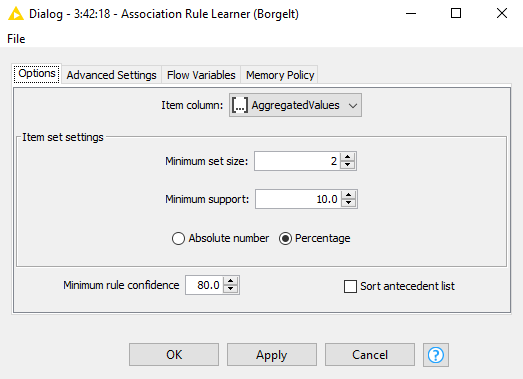
\includegraphics[width=\linewidth]{figuras/Jenn/config-assoc-rules}
		\caption{Configuración del nodo \textit{Association Rule Learner (BorgeIt)}}
		\label{fig:conf-assoc-rules}
	\end{subfigure}
	\hfill
	\begin{subfigure}[b]{0.4\linewidth}
		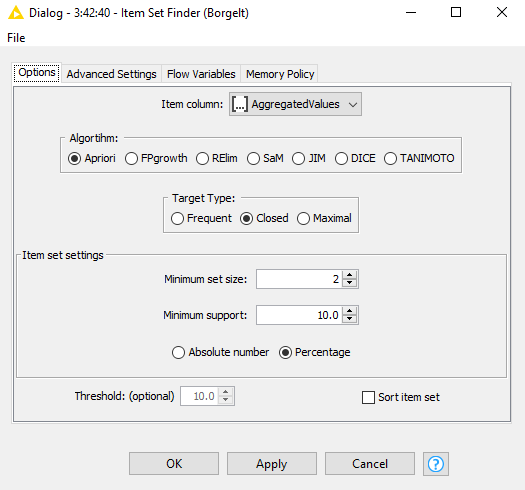
\includegraphics[width=\linewidth]{figuras/Jenn/conf-itemset}
		\caption{Configuración del nodo \textit{Item Set Finder (BorgeIt)}}
		\label{fig:config-itemset}
	\end{subfigure}
	\caption{Configuración de los nodos para la obtención de reglas de asociación}
	\label{fig:conf-reglas}
\end{figure}

Las reglas de asociación obtenidas para el conjunto de \textsc{Alto Riesgo} están presentes en la figura \ref{fig:reglas-train}, donde todos los consecuentes equivalen al valor \textsc{SI}, es decir, al fraude.

\begin{figure}[H]
	\centering
	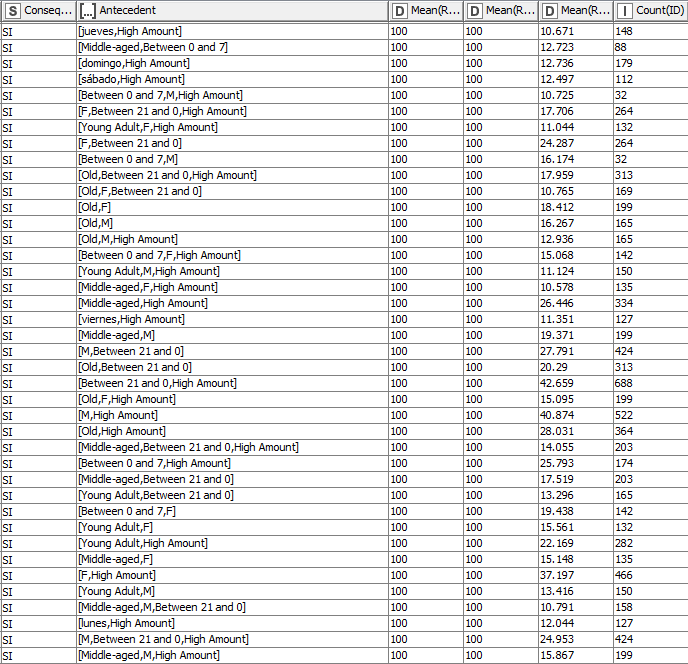
\includegraphics[width=0.6\linewidth]{figuras/Jenn/reglas-train}
	\caption{Reglas de asociación obtenidas de los clústeres de \textsc{Alto Riesgo}}
	\label{fig:reglas-train}
\end{figure}


\subsubsection{Conclusiones del agrupamiento y reglas de asociación}

Tras el análisis de las reglas de asociación obtenidas en el análisis de los grupos de alto riesgo, así como de los resultados de agrupamiento, se puede concluir que:
\begin{itemize}
	\item Existe un clúster donde se agrupa cerca de un 46\% de transacciones fraudulentas con respecto al total de ambas bases de datos (entrenamiento y prueba), y que, además, se encuentran menos del 1\% de transacciones legítimas.
	\item La mayoría de las transacciones fraudulentas ocurren en el intervalo de 9.00p.m. y 12.00a.m., con un monto alto, es decir mayor a \$90 y menor a \$10 000.
	\item Muchas de las transacciones fraudulentas son originadas por personas de media edad o edad avanzada, es decir mayor a 26 años.
	\item Los días donde más ocurren transacciones fraudulentas son jueves, sábado y domingo.
\end{itemize}


\section{Conclusiones parciales}
Al finalizar este capítulo, se llega a las siguientes conclusiones:

\begin{itemize}
	\item Se realizaron varias pruebas en la tarea de clasificación, donde se emplearon árboles de decisión y bosques aleatorios.
	\item Ambos clasificadores demostraron más de un 65\% de clasificación exitosa con respecto a las transacciones fraudulentas.
	\item Se obtuvo un modelo de agrupamiento que obtuvo un clúster con una gran proporción de transacciones fraudulentas, con respecto al total existente en la base de datos de pruebas.
	\item Se obtuvieron reglas de asociación relevantes de acuerdo al clúster donde se presentaba un mayor número de transacciones fraudulentas, con un 90\% de confianza mínima y un soporte mínimo del 10\%.
\end{itemize}

\pagebreak
